\documentclass[10pt,a4paper]{article}

\usepackage[margin=0.75in]{geometry}
\usepackage[T1]{fontenc}
\usepackage[utf8]{inputenc}
\usepackage{lmodern}
\usepackage{graphicx}
\usepackage{booktabs}
\usepackage{array}
\usepackage{float}
\usepackage{hyperref}
\usepackage{caption}

\hypersetup{
    colorlinks=true,
    urlcolor=blue,
    linkcolor=black
}

\setlength{\parskip}{0.45em}
\setlength{\parindent}{0pt}
\captionsetup{font=small}

\begin{document}

\begin{center}
{\Large \textbf{Data Mining Assignment 2: Recommender Systems}}\\[0.4em]
\normalsize Simple Movie Recommendation Report\\[0.3em]
\small GitHub repository: \url{https://github.com/alperendavran/assigment-2-alperen-davran-data-mining}
\end{center}

\section*{1. Introduction}
The goal of this assignment is to build and compare recommender models for movie recommendation, and then generate 10 recommendations for each user in \texttt{ratings\_test.csv}. I focused on the two things that the assignment asks for most clearly:

\begin{itemize}
\item rating prediction quality, measured with \texttt{RMSE}
\item top-10 recommendation quality, measured mainly with \texttt{Precision@10} and \texttt{Recall@10}
\end{itemize}

I compared three models: a bias-based baseline, a user-based collaborative filtering model, and an SVD matrix factorization model. The final system also had to handle cold-start users, because some users in the test file do not appear in the training data.

\section*{2. Data Understanding And Preprocessing}
The training data contains \texttt{97,801} ratings from \texttt{600} users on \texttt{9,680} movies. The user-item matrix is about \texttt{98.32\%} sparse, so most possible user-movie pairs are missing. This is important because sparse data usually makes neighborhood methods less stable and gives more room for latent-factor methods to help.

Some other statistics are also useful:

\begin{itemize}
\item average ratings per user: \texttt{163.0}, median: \texttt{69.5}
\item average ratings per movie: \texttt{10.1}, median: \texttt{3.0}
\item share of ratings from the top \texttt{10\%} most-rated movies: \texttt{59.66\%}
\item movies with zero training ratings: \texttt{62}
\end{itemize}

These numbers show a clear long-tail structure. A small set of movies gets many ratings, while most movies receive only a few. Because of that, popular movies are easier to recover, so popularity-heavy recommendations can look stronger than expected.

During preprocessing, I checked missing values, duplicate user-movie ratings, and the rating range. No missing values and no duplicate ratings were found. I also added simple movie statistics such as average rating and rating count, which were later useful for analysis and for the cold-start fallback.

\begin{figure}[H]
    \centering
    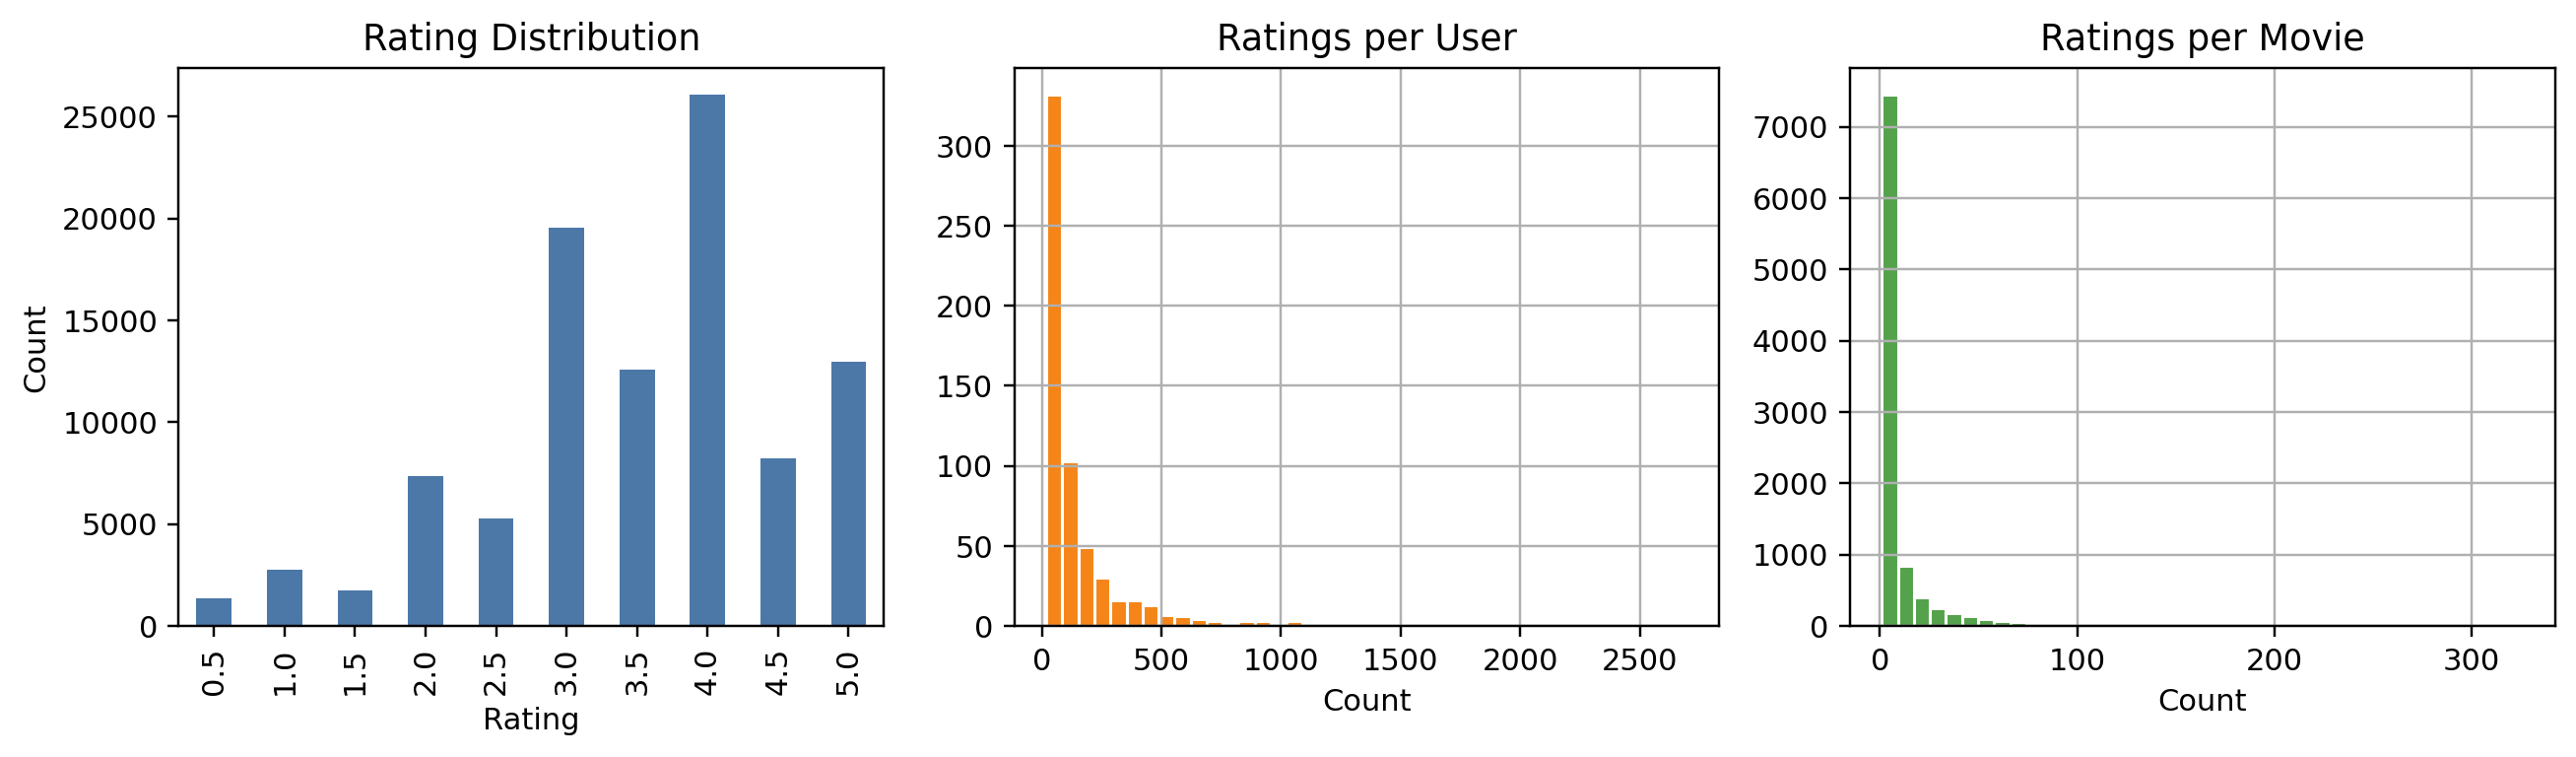
\includegraphics[width=\linewidth]{report_assets/data_overview.png}
    \caption{Basic data overview. The plots show rating concentration, uneven user activity, and a strong long-tail on the movie side.}
\end{figure}

Finally, I checked whether the users in \texttt{ratings\_test.csv} were present in the training data. There were \texttt{90} warm users and \texttt{10} cold-start users, so \texttt{10\%} of the final recommendations required a fallback strategy.

\section*{3. Models And Evaluation Setup}
For validation, I used a temporal split. For each user, the ratings were sorted by timestamp and the last \texttt{5} interactions were held out. The remaining ratings were used for training. I chose this because the timestamps make it possible to respect interaction order instead of using a fully random split.

For ranking evaluation, only held-out ratings of \texttt{4.0} or higher were treated as relevant items. In this setup, \texttt{1,696} held-out ratings were relevant, and \texttt{533} out of \texttt{600} users had at least one relevant held-out item. This means \texttt{88.83\%} of users contributed to the ranking evaluation.

The three models were:

\textbf{Baseline.} This model predicts ratings from the global mean together with user and item bias terms. It gives a simple reference point and helps separate real collaborative effects from global popularity and bias effects. In Surprise, this is \texttt{BaselineOnly}, which predicts from \texttt{$\mu + b_u + b_i$} \cite{surprise-basic}.

\textbf{User-based collaborative filtering.} This model estimates a user's preference from similar users. It is intuitive and easy to explain, but it depends strongly on overlap between users. In sparse data, that overlap can be weak.

\textbf{SVD matrix factorization.} This model learns latent user and item factors together with bias terms. It is a standard matrix factorization approach and is often more suitable for sparse recommender data because it does not rely as directly on local user-user overlap \cite{koren2009,surprise-svd}.

I reported \texttt{RMSE}, \texttt{Precision@10}, and \texttt{Recall@10} as the main metrics because they match the assignment most directly. I kept \texttt{HR@10} and \texttt{NDCG@10} as supporting metrics only.

The general idea behind top-$N$ lists and precision/recall at $K$ matches the explanations in the Surprise FAQ \cite{surprise-faq}. My validation setup uses a temporal holdout and sampled negatives, so it is not identical to the library examples, but the metric definitions are consistent with that reference.

\section*{4. Results And Discussion}
The main validation results are shown in Table~\ref{tab:main-results}.

\begin{table}[H]
\centering
\caption{Main validation results}
\label{tab:main-results}
\small
\begin{tabular}{lrrrrrr}
\toprule
Model & RMSE & P@10 & R@10 & HR@10 & NDCG@10 & Time \\
\midrule
Baseline & 0.9389 & 0.0756 & 0.2255 & 0.5488 & 0.1761 & 0.3 \\
User-Based CF & 0.9398 & 0.0370 & 0.1137 & 0.3114 & 0.0711 & 1.8 \\
SVD & 0.9366 & 0.0638 & 0.1894 & 0.4883 & 0.1424 & 0.4 \\
\bottomrule
\end{tabular}
\end{table}

At first glance, the baseline looks surprisingly strong, especially on \texttt{Recall@10}. I think a likely explanation is the long-tail structure of the data. Since nearly \texttt{60\%} of all ratings come from the top \texttt{10\%} most-rated movies, popular items are easier to recover. A model that captures global movie effects can therefore perform well on ranking metrics even without much personalization.

To make this trade-off more visible, I also compared the recommendation lists themselves across \texttt{50} sampled users.

\begin{table}[H]
\centering
\caption{Recommendation statistics over 50 sampled users}
\small
\begin{tabular}{lrrr}
\toprule
Model & Coverage & Avg. popularity & Max repeat \\
\midrule
Baseline & 43 & 129.4 & 46 \\
User-Based CF & 252 & 14.1 & 15 \\
SVD & 160 & 88.1 & 17 \\
\bottomrule
\end{tabular}
\end{table}

\begin{figure}[H]
    \centering
    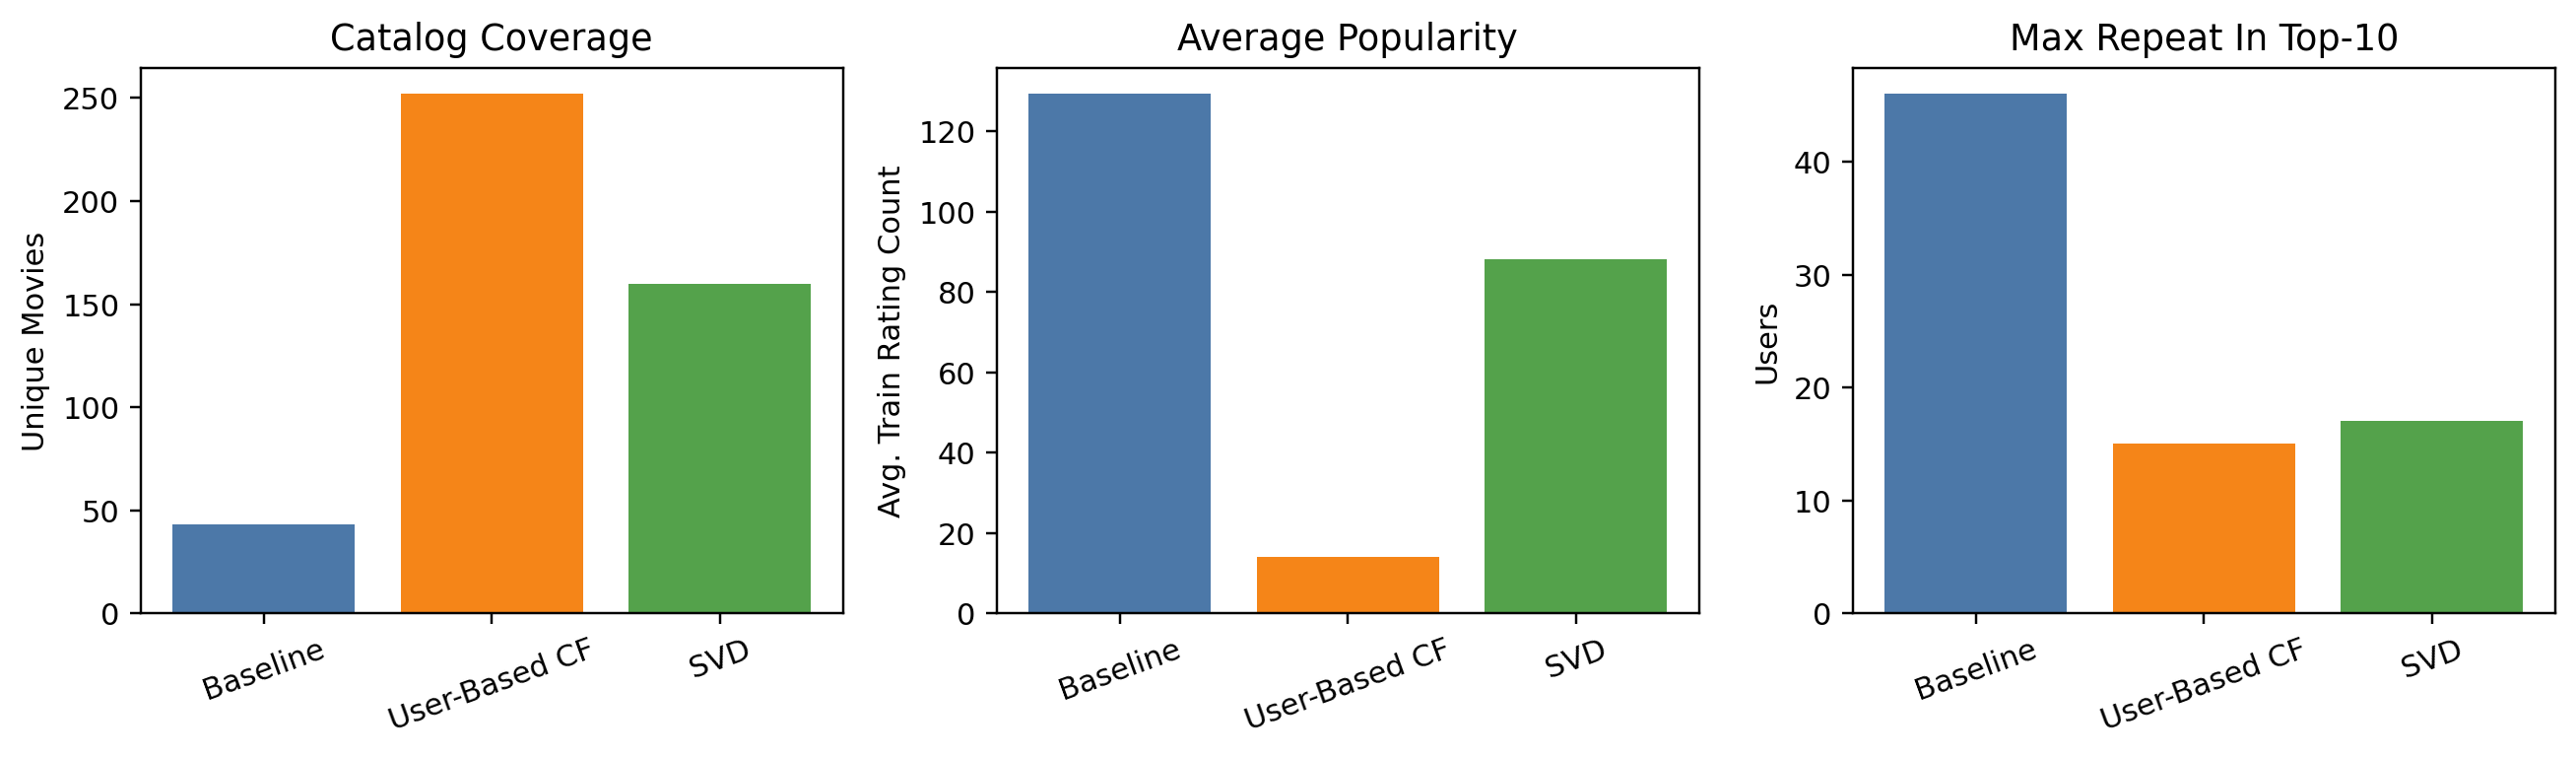
\includegraphics[width=\linewidth]{report_assets/recommendation_stats.png}
    \caption{The baseline is strong but highly concentrated, while SVD gives a broader recommendation set without collapsing to extremely niche items.}
\end{figure}

These results help explain the model behavior more clearly. The baseline repeats the same popular movies for many users. The user-based model is much more personalized, but its accuracy is clearly weaker. SVD sits between the two and gives a more convincing compromise.

In this dataset, the user-based model suffers from the data structure itself: the matrix is about \texttt{98\%} sparse and the median movie has only \texttt{3} ratings, so user-user overlap is often too limited for stable neighborhoods. SVD gives the best \texttt{RMSE}, clearly better ranking performance than the user-based model, and much broader coverage than the baseline. For that reason, I selected SVD as the final personalized model.

I also tested a small hyperparameter search for SVD. However, it was optimized for \texttt{RMSE} on random folds and did not improve \texttt{Precision@10} or \texttt{Recall@10} on the temporal validation setup, so I did not use it as the final model.

\section*{5. Final Recommendation Strategy}
For the final recommendation step, I retrained SVD on the full training set and generated the top \texttt{10} unseen movies for each warm user.

The final pipeline handled two cases:

\begin{itemize}
\item \textbf{Warm users:} score all unseen movies with SVD and return the top \texttt{10}
\item \textbf{Cold-start users:} return a popularity-based fallback list
\end{itemize}

The fallback was needed for \texttt{10} out of \texttt{100} test users. For those users, collaborative filtering cannot personalize recommendations because there is no interaction history. Instead of using a plain average rating, I used a weighted rating formula so that movies with only a few ratings would not look artificially strong.

This is not a perfect solution to the cold-start problem, but it is simple, transparent, and reasonable for the scope of the assignment.

\section*{6. Conclusion}
This dataset is challenging because it is highly sparse and strongly long-tail. Those properties make popularity-based recommendations look stronger than expected and make user-based neighborhoods less stable.

Among the tested models, SVD was the most suitable final personalized model for this assignment. It had the strongest \texttt{RMSE}, better ranking results than user-based CF, and much broader recommendation coverage than the baseline. The final system therefore uses SVD for warm users and a weighted popularity fallback for cold-start users.

I do not claim that this fully solves recommendation quality or cold-start. However, I think it is a logical and well-motivated solution for the scope of the assignment.

As future work, a hybrid approach such as LightFM could combine collaborative signals with movie metadata (for example genres) \cite{lightfm}. That direction is appealing for cold-start items, but the official examples often emphasize implicit feedback, whereas this assignment also requires explicit rating error in the form of \texttt{RMSE}, so I kept the main experiments on Surprise-based models.

\begin{thebibliography}{9}

\bibitem{koren2009}
Y. Koren, R. Bell, and C. Volinsky.
\newblock Matrix factorization techniques for recommender systems.
\newblock \emph{Computer}, 42:30--37, 2009.
\newblock \url{https://www.chrisvolinsky.com/publications/17545-matrix-factorization-techniques-for-recommender-systems}

\bibitem{surprise-svd}
Surprise documentation.
\newblock Matrix factorization-based algorithms.
\newblock \url{https://surprise.readthedocs.io/en/stable/matrix_factorization.html}

\bibitem{surprise-basic}
Surprise documentation.
\newblock Basic algorithms.
\newblock \url{https://surprise.readthedocs.io/en/stable/basic_algorithms.html}

\bibitem{surprise-faq}
Surprise documentation.
\newblock FAQ: top-$N$ recommendations and precision/recall at $K$.
\newblock \url{https://surprise.readthedocs.io/en/stable/FAQ.html}

\bibitem{lightfm}
LightFM documentation.
\newblock Hybrid matrix factorization models.
\newblock \url{https://making.lyst.com/lightfm/docs/home.html}

\end{thebibliography}

\end{document}
